\section{定积分的应用}

对于非均匀分布的物理量的累积,可以用定积分求解,关键是建立积分表达式——微元法。
微元法把物理量分割成一个个小量——微元,每个微元内近似分布均匀,对这个分布均匀的微元列出表达式,最后积分。

本节要点:
\begin{itemize}
    \item 通过3个例子体会定积分的应用及使用方法;
    \item 了解平均值和均方根值的概念。
\end{itemize}

\begin{tcolorbox}
注意,微元法中,我们先微分再积分,体会这个矛盾统一体。
\end{tcolorbox}

%============================================================
\subsection{变力作功}

\begin{example}
假设弹簧的胡克系数$k$,从放松状态拉长$l$,需做多少功?
\end{example}

解:

根据功的定义$W=F\cdot S$,对拉长微元$dx$内可以认为力$F\left( x \right) =kx$不变,该拉长微元下功的微元$dW=F\left( x \right) dx=kx\cdot dx$,于是,整体作功:
\[
W=\int_0^l{dW}=\int_0^l{kx\cdot dx}=\left. \frac{1}{2}kx^2 \right|_{0}^{l}=\frac{1}{2}kl^2
\]

%============================================================
\subsection{一维物体引力}

\begin{example}
小球质量$m$,均匀细长杆质量$M$、长$L$、重量均匀且密度为$\mu $,小球位于细长杆延长线,距细长杆$d$,求小球受到的引力。
\begin{figure}[h]
\centering
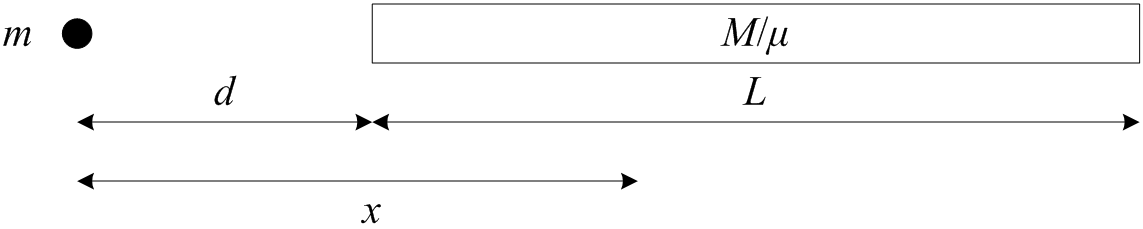
\includegraphics[height=1.5cm]{3.5.png}
\end{figure}
\end{example}

解:

小球可以视为质点,但细长杆不行,根据引力方程,假设细长杆的一个微元对小球的引力可以视为质点,则引力微元$dF=G\frac{m\cdot \mu dx}{x^2}$,整体引力:
\begin{align*}
F&=\int_d^{d+L}{G\frac{m\cdot \mu dx}{x^2}}=Gm\mu \int_d^{d+L}{\frac{1}{x^2}\cdot dx} \\
&=Gm\mu \left( \left. -\frac{1}{x} \right|_{d}^{d+L} \right) =Gm\mu \left( \frac{1}{d}-\frac{1}{d+L} \right)
\end{align*}

%============================================================
\subsection{第二宇宙速度}

\begin{example}
求第二宇宙速度,即脱离地球引力范围的最小速度。
\end{example}

解:

假设地球质量$M$,物体质量$m$,地球半径$R$,脱离地球引力范围即相当于飞至无限远。
结合能量守恒定律,物体飞至无限远引力做功即物体的初动能:
\[
\frac{1}{2}{mv_0}^2=\int_R^{+\infty}{F\left( r \right) dr}=\int_R^{+\infty}{G\frac{Mm}{r^2}dr}
\]
该问题从数学上看是一个无穷区间上的反常积分:
\begin{align*}
&\because \int_R^{+\infty}{G\frac{Mm}{r^2}dr}=GMm\left( \left. -\frac{1}{r} \right|_{R}^{+\infty} \right) =\frac{GMm}{R} \\
&\therefore v_0=\sqrt{\frac{2GM}{R}}=\sqrt{2gR}\approx 11.2\mathrm{km}/\mathrm{s}
\end{align*}
物体的初速度11.2km/s,即为第二宇宙速度。

%============================================================
\subsection{函数的平均值和均方根值}

之前我们讨论了离散量的算术平均值:
\[
\bar{x}=\frac{x_1+x_2+\cdots +x_n}{n}
\]
如果是连续量,如电流、功率,就涉及连续函数的平均值。

\begin{definition}[函数的平均值]
设函数$f\left( x \right) $在$\left[ a,b \right] $上连续,将$\left[ a,b \right] $等分为$n$个小区间$a=x_0<x_1<x_2<...<x_{n-1}<x_n=b$,记每个小区间的长度$\Delta x_i=\frac{b-a}{n}$,我们可以用:
\[
\frac{f\left( x_1 \right) +f\left( x_2 \right) +\cdots +f\left( x_n \right)}{n}=\frac{1}{n}\sum_{i=1}^n{f\left( x_i \right)}
\]
近似描述平均值,如果当$n\rightarrow \infty $时该和式有极限,我们就称该极限为{\bf 函数$f\left( x \right) $在$\left[ a,b \right] $上的平均值},记作$\bar{y}$,即:
\begin{align*}
\bar{y}:&=\underset{n\rightarrow \infty}{\lim}\frac{1}{n}\sum_{i=1}^n{f\left( x_i \right)}=\underset{n\rightarrow \infty}{\lim}\sum_{i=1}^n{\frac{f\left( x_i \right)}{n}} \\
&=\underset{n\rightarrow \infty}{\lim}\sum_{i=1}^n{\left[ f\left( x_i \right) \cdot \frac{\Delta x_i}{b-a} \right]}=\frac{1}{b-a}\underset{n\rightarrow \infty}{\lim}\sum_{i=1}^n{\left[ f\left( x_i \right) \cdot \Delta x_i \right]} \\
&=\frac{1}{b-a}\int_a^b{f\left( x \right) dx}
\end{align*}
\end{definition}

\begin{definition}[函数的均方根值]

若函数$f\left( x \right) $在$\left[ a,b \right] $上连续,我们称如下积分为{\bf 函数$f\left( x \right) $在$\left[ a,b \right] $上的均方根值},常记作RMS(Root Mean Square),即:
\[
RMS:=\sqrt{\frac{1}{b-a}\int_a^b{f^2\left( x \right) dx}}
\]
\end{definition}

物理上,我们通常用平均值表示一个物理量一段时间内的平均值,特别是周期物理量,用均方根值表示物理量的有效值。

~

\begin{example}
若交流电的电流$I\left( t \right) =I_m\sin \omega t$,$I_m$为峰值,计算在电阻$R$上的平均功率和有效电流。
\end{example}

解:

交流电的平均功率可以计算在一个周期$T=2\pi /\omega $内的功率的平均值,如下:
\begin{align*}
&\because P\left( t \right) =I^2\left( t \right) R=\left( I_m\sin \omega t \right) ^2R \\
&\therefore \bar{P}=\frac{1}{T}\int_0^T{P\left( t \right) dt}=\frac{\omega}{2\pi}\int_0^{2\pi /\omega}{\left( I_m\sin \omega t \right) ^2R\cdot dt}=\frac{1}{2}{I_m}^2R
\end{align*}
有效电流采用均方根值计算方式:
\[
\sqrt{\frac{1}{T}\int_0^T{I^2\left( t \right) \cdot dt}}=\sqrt{\frac{\omega}{2\pi}\int_0^{2\pi /\omega}{\left( I_m\sin \omega t \right) ^2\cdot dt}}=\frac{1}{\sqrt{2}}I_m
\]




